\documentclass[../main.tex]{subfiles}
\graphicspath{{\subfix{../images/}}}


\begin{document}
% AIS
%%%%%%%%%%%%%%%%%%%%%%%%%%%%%%%%%%%%%%%%%%%%%%%%%%%%%%%%%%%%%%%%%%%%%%%%%%%%%%%
Vessels navigating the Baltic Sea

Importance of maritime traffic globally and timely operation


\subsection{Automatic identification system}

What is AIS, what is is features, problems. Example of raw AIS data.

\subsubsection{Estimated Time of Arrival}

Importance of ETA and what current systems there is.

\subsection{HELCOM dataset}

Introduction to HELCOM

Describe the features and quirks with the HELCOM dataset as it is a processed dataset that contains AIS data already processed from the raw format.

Showing examples of the data as plots of the Baltic, also shows the area covered

\begin{figure}[h]
\centering
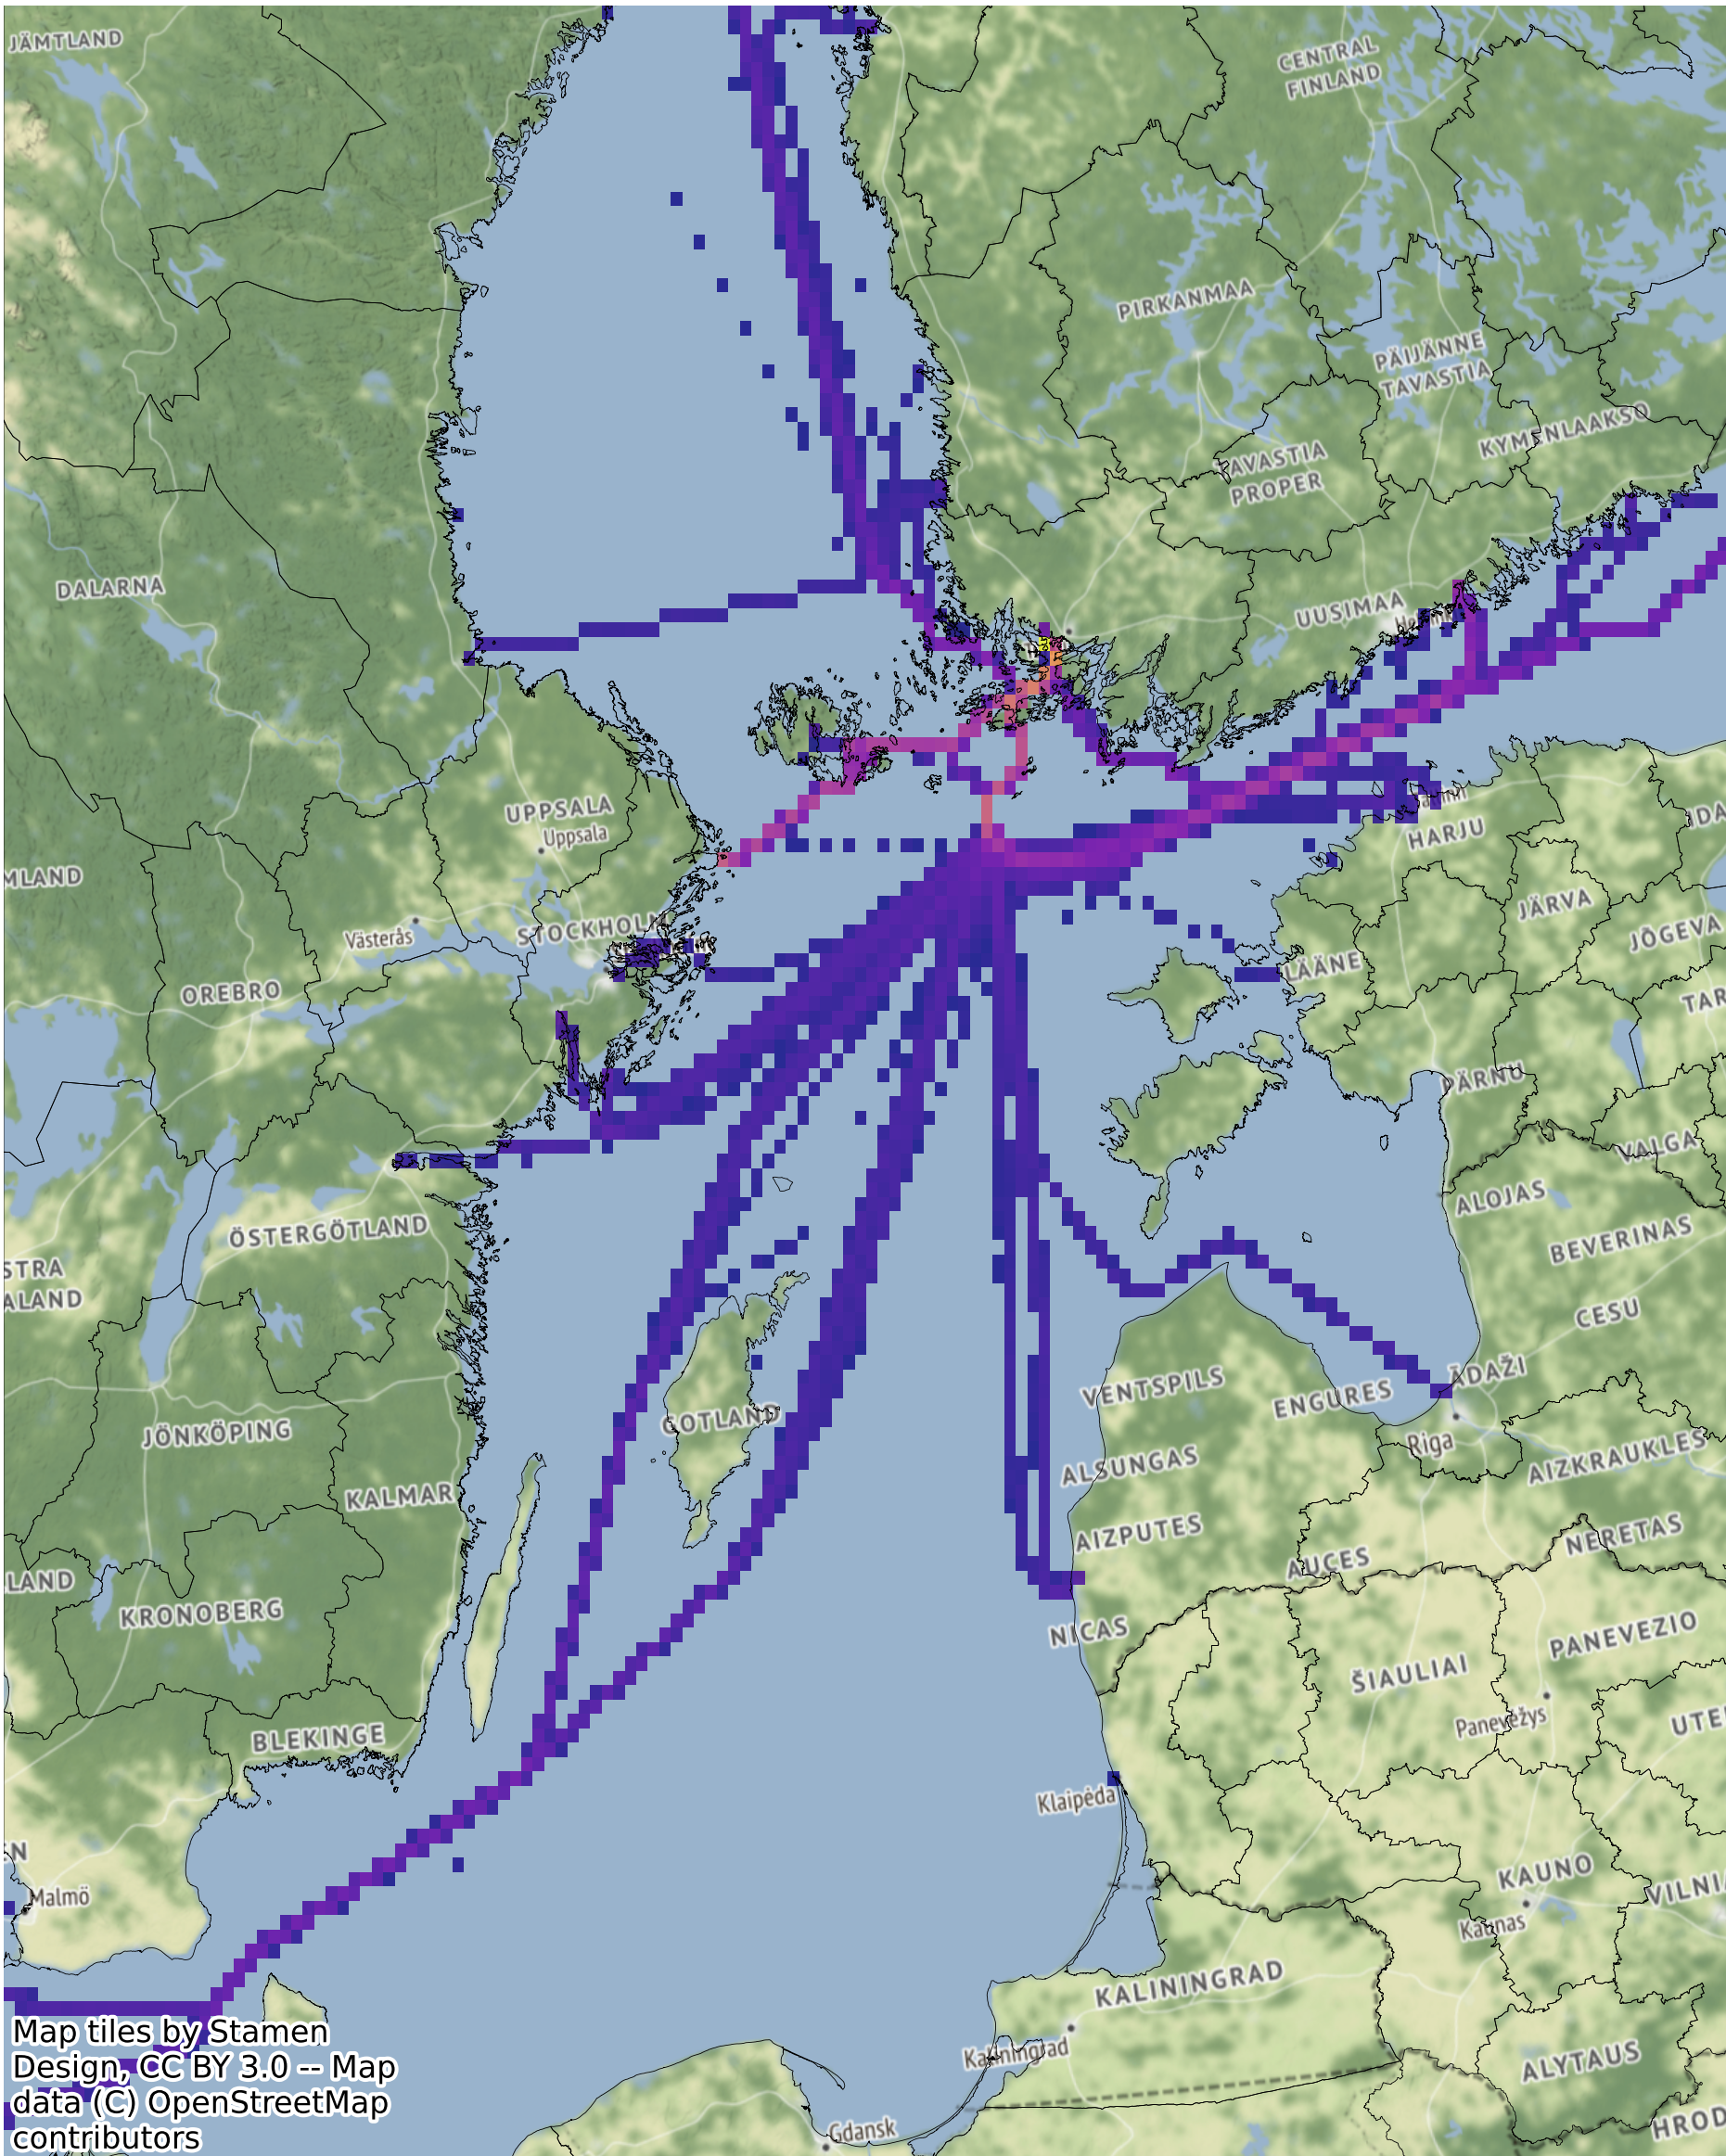
\includegraphics[scale=.3]{heatmap-train-data-13-03.png}
\caption{Heatmap the Baltic Sea with a limit of more than 10 unique messages per grid cell.}
\label{fig:heatmap}
\end{figure}

\subsubsection{Description of HELCOM dataset features}

\subsubsection{Statistical information}

Vessels physical features and the grouping of different vessels by size.

\subsection{Port of Naantali}

The amount of data collected travelling to FINLI from the HELCOM dataset, rather busy port approx. 2 \% of the total data per month

\end{document}